
% In the remain part of this paper, we investigate how the {\color{cc1}optimization} (Section~\ref{sec4}), {\color{cc2}data distribution} (Section~\ref{sec5}), {\color{cc3}loss function} (Section~\ref{sec6}), and {\color{cc4}model architecture} (Section~\ref{sec7}) influence the emergence of attention sink by pre-training hundreds of LMs.

% \begin{equation}
% {\color{cc1}\min_{\theta}}\hspace{0.05cm}\mathbb{E}_{{\color{cc2}\boldsymbol{X}\sim p_{\textrm{data}}}}\left[{\color{cc3}\mathcal{L}}\left({\color{cc4}p_{\theta}}(\boldsymbol{X})\right)\right]\textrm{.}
% \end{equation}

\vspace{-0.2cm}
\section{Effects of {\color{cc4}model architecture \texorpdfstring{$p_{\theta}$}{TEXT}} on attention sink}
\vspace{-0.2cm}
\label{sec7}

In this section, we mainly explore the effects of positional embedding, pre-norm or post-norm structure, and attention design on the emergence of attention sink. In Appendix~\ref{appendix_model}, we also show that varying activation functions in the FFN, multi-head design do not affect the emergence of attention sink.\looseness=-1

\vspace{-0.15cm}
\subsection{Positional embedding}
\vspace{-0.15cm}


Attention sink always appears on the first token, which motivates us to explore where such a position property is brought by positional embedding (PE). Therefore, we attempt to replace the original Rotary with other PEs, as shown in Table~\ref{pe}. We differentiate these PEs through the calculations of the hidden states $\boldsymbol{H}^0$ before the first transformer block and the dot product between queries and keys $\langle\boldsymbol{q}_i\textrm{,}\,\boldsymbol{k}_j\rangle$. The detailed formulations are delayed to Appendix~\ref{appendix_llm}. From the same Table, we observe that only the model with relative PE is difficult to train while other models have comparable performance under our setup. Then we note that all these LMs, even the one without explicit PE (NoPE), have attention sink.\looseness=-1



% Although NoPE does not explicitly encode either absolute or relative positions, the token positions are already implicitly encoded through the casual mask.  We summarize these PEs in Table~\ref{pe} and delay the detailed formulations in Appendix~\ref{appendix_llm}.


% NoPE~\citep{kazemnejad2024impact}, absolute PE (APE)~\citep{vaswani2017attention, Brown2020language}, learnable PE (LPE)~\citep{devlin2019bert}, relative PE (RPE)~\citep{raffel2020exploring}, and ALiBi~\citep{press2021train}.


% \begin{table}[htbp]
% \begin{center}
% \begin{tabular}{l|cccccc}
% \toprule
% PE & NoPE & APE & LPE & RPE & AliBi & RoPE \\
% \midrule
% $\boldsymbol{P}$ & $\boldsymbol{0}$ & $\boldsymbol{P}$ & $\boldsymbol{P}$ & $\boldsymbol{0}$  & $\boldsymbol{0}$ & $\boldsymbol{0}$ \\
% % \midrule
% $\langle\boldsymbol{q}_i\textrm{,}\,\boldsymbol{k}_j\rangle$ & $\boldsymbol{q}_i^T\boldsymbol{k}_j$ & $\boldsymbol{q}_i^T\boldsymbol{k}_j$ & $\boldsymbol{q}_i^T\boldsymbol{k}_j$ & $\boldsymbol{q}_i^T\boldsymbol{k}_j+g(i-j)$ & $\boldsymbol{q}_i^T\boldsymbol{k}_j+g(i-j)$ & $\boldsymbol{q}_i^T\boldsymbol{R}_{\Phi\textrm{,}\,j-i}\boldsymbol{k}_j$ \\
% \bottomrule
% \end{tabular}
% \end{center}
% \vspace{-.2cm}
% \caption{Positional Embedding.}
% \vspace{-.2cm}
% \label{pe}
% \end{table}

% \begin{table}[htbp]
% \begin{center}
% \begin{tabular}{l|llcccc}
% \toprule
% PE & $\boldsymbol{H}^0$ & $\langle\boldsymbol{q}_i\textrm{,}\,\boldsymbol{k}_j\rangle$ & $\alpha_1$ &  $\beta$ & valid loss\\
% \midrule

% NoPE & $\boldsymbol{X}\boldsymbol{W}_E$ & $\boldsymbol{q}_i^T\boldsymbol{k}_j$ & 25.83 & 3.92 & 3.81\\
% APE & $\boldsymbol{X}\boldsymbol{W}_E+\boldsymbol{P}$ & $\boldsymbol{q}_i^T\boldsymbol{k}_j$ & 36.39 & 5.41 & 3.74\\
% LPE & $\boldsymbol{X}\boldsymbol{W}_E+\boldsymbol{P}$ & $\boldsymbol{q}_i^T\boldsymbol{k}_j$ & 35.88 & 5.03 & 3.79\\
% RPE & $\boldsymbol{X}\boldsymbol{W}_E$ & $\boldsymbol{q}_i^T\boldsymbol{k}_j+g(i-j)$ & 36.73 & 3.18 & 5.45\\
% ALiBi & $\boldsymbol{X}\boldsymbol{W}_E$ & $\boldsymbol{q}_i^T\boldsymbol{k}_j+g(i-j)$ & 23.73 & 3.61 & 3.71\\
% RoPE & $\boldsymbol{X}\boldsymbol{W}_E$ & $\boldsymbol{q}_i^T\boldsymbol{R}_{\Phi\textrm{,}\,j-i}\boldsymbol{k}_j$ & 21.30 & 3.52 & 3.73\\

% \bottomrule
% \end{tabular}
% \end{center}
% \vspace{-.2cm}
% \caption{Positional Embedding.}
% \vspace{-.2cm}
% \label{pe}
% \end{table}


% \begin{table}[htbp]
% \begin{center}
% \begin{tabular}{l|cccccc}
% \toprule
% Positional Embedding & NoPE & APE & Learnable PE & Relative PE & AliBi & RoPE \\
% \midrule
% $\alpha_1$ (\%) & 25.83 & 36.39 & 35.88 & 36.73 & 23.73 & 21.30\\
% % \midrule
% $\beta_1$ & 3.92 & 5.41 & 5.03 & 3.18 & 3.61 & 3.52 \\
% Valid loss & 3.81 & 3.74 & 3.79 & 5.45 & 3.71 & 3.73  \\
% \bottomrule
% \end{tabular}
% \end{center}
% \vspace{-.2cm}
% \caption{Positional Embedding.}
% \vspace{-.2cm}
% \label{pe}
% \end{table}



% \textbf{Model Depth.}



% \begin{table}[htbp]
% \begin{center}
% \begin{tabular}{l|lccc}
% \toprule
% Activations & $\boldsymbol{F}$ & $\alpha$ &  $\beta$ & valid loss \\
% \midrule

% ReLU & $\textrm{ReLU}(\boldsymbol{h}\boldsymbol{W}_1)\boldsymbol{W}_2$ & 22.62 & 3.16 & 3.82\\
% GeLU & $\textrm{GeLU}(\boldsymbol{h}\boldsymbol{W}_1)\boldsymbol{W}_2$ & 19.86   & 3.07 & 3.79 \\
% Swish & $\textrm{Swish}(\boldsymbol{h}\boldsymbol{W}_1)\boldsymbol{W}_2$ &  24.30 &3.41  & 3.80 \\
% ReGLU & $\left(\textrm{ReLU}(\boldsymbol{h}\boldsymbol{W}_1)\odot\boldsymbol{h}\boldsymbol{W}_2\right)\boldsymbol{W}_3$ & 19.15 & 3.10 & 3.75\\
% GeGLU & $\left(\textrm{GeLU}(\boldsymbol{h}\boldsymbol{W}_1)\odot\boldsymbol{h}\boldsymbol{W}_2\right)\boldsymbol{W}_3$ &  21.87 & 3.43 & 3.73\\
% SwiGLU & $\left(\textrm{Swish}(\boldsymbol{h}\boldsymbol{W}_1)\odot\boldsymbol{h}\boldsymbol{W}_2\right)\boldsymbol{W}_3$ &  21.30 & 3.52 & 3.73\\

% \bottomrule
% \end{tabular}
% \end{center}
% \vspace{-.2cm}
% \caption{Activations in FFN.}
% \vspace{-.2cm}
% \label{activation}
% \end{table}

\vspace{-0.2cm}
\subsection{Pre-norm and post-norm structure} 
\vspace{-0.2cm}
Layer normalization (LN)~\citep{ba2016layernormalization,zhang2019root} regularizes the hidden states in LMs by re-centering and re-scaling, which may affect the massive activations. This motivates us to explore the effects of LN location on attention sink. In the pre-norm structure, as stated in \Eqref{eq-pre-norm}, hidden states from the earlier blocks could be retained by the later blocks through residual connections~\citep{he2016deep}.  Therefore, if massive activations appear in a specific block, they will likely be retained in the subsequent blocks. Within a post-norm structure, the hidden states will be normalized before being fed into the following blocks, as present in Figure~\ref{architecture}(\emph{Left}). 

When replacing the pre-norm structure with the post-norm structure, $\textrm{Sink}_1^{\epsilon}$ becomes 13.54\%. This indicates that the attention sink still exists in post-norm LMs. After further investigations, as visualized in Figure~\ref{massive_activations}(\emph{Left}), massive activations exist in the hidden states before the post LN instead of $\boldsymbol{h}_1^{l}$.\looseness=-1 


\begin{table}[t]
\vspace{-1cm}
\caption{Positional embedding does not affect the emergence of attention sink.}
\vspace{-.5cm}
\begin{center}
\begin{tabular}{l|ll|ccc}
\toprule
PE & $\boldsymbol{H}^0$ & $\langle\boldsymbol{q}_i\textrm{,}\,\boldsymbol{k}_j\rangle$ & $\textrm{Sink}_1^{\epsilon}$(\%)  & valid loss\\
\midrule
NoPE & $\boldsymbol{X}\boldsymbol{W}_E$ & $\boldsymbol{q}_i\boldsymbol{k}_j^\top$ & 20.35 & 3.81\\
Absolute PE & $\boldsymbol{X}\boldsymbol{W}_E+\boldsymbol{P}_{\textrm{abs}}$ & $\boldsymbol{q}_i\boldsymbol{k}_j^\top$ & 32.73 &  3.74\\
Learnable PE & $\boldsymbol{X}\boldsymbol{W}_E+\boldsymbol{P}_{\textrm{learnable}}$ & $\boldsymbol{q}_i\boldsymbol{k}_j^\top$ & 33.13 &  3.79\\
Relative PE & $\boldsymbol{X}\boldsymbol{W}_E$ & $\boldsymbol{q}_i\boldsymbol{k}_j^\top+g_{\textrm{relative}}(i-j)$ & 35.53 & 5.45\\
ALiBi & $\boldsymbol{X}\boldsymbol{W}_E$ & $\boldsymbol{q}_i\boldsymbol{k}_j^\top+g_{\textrm{alibi}}(i-j)$ & 20.78 &  3.71\\
Rotary & $\boldsymbol{X}\boldsymbol{W}_E$ & $\boldsymbol{q}_i\boldsymbol{R}_{\Theta\textrm{,}\,j-i}\boldsymbol{k}_j^\top$ & 18.18 & 3.73\\
\bottomrule
\end{tabular}
\end{center}
\vspace{-.3cm}
\label{pe}
\end{table}

\begin{figure}[t]
\centering
\vspace{-0.25cm}
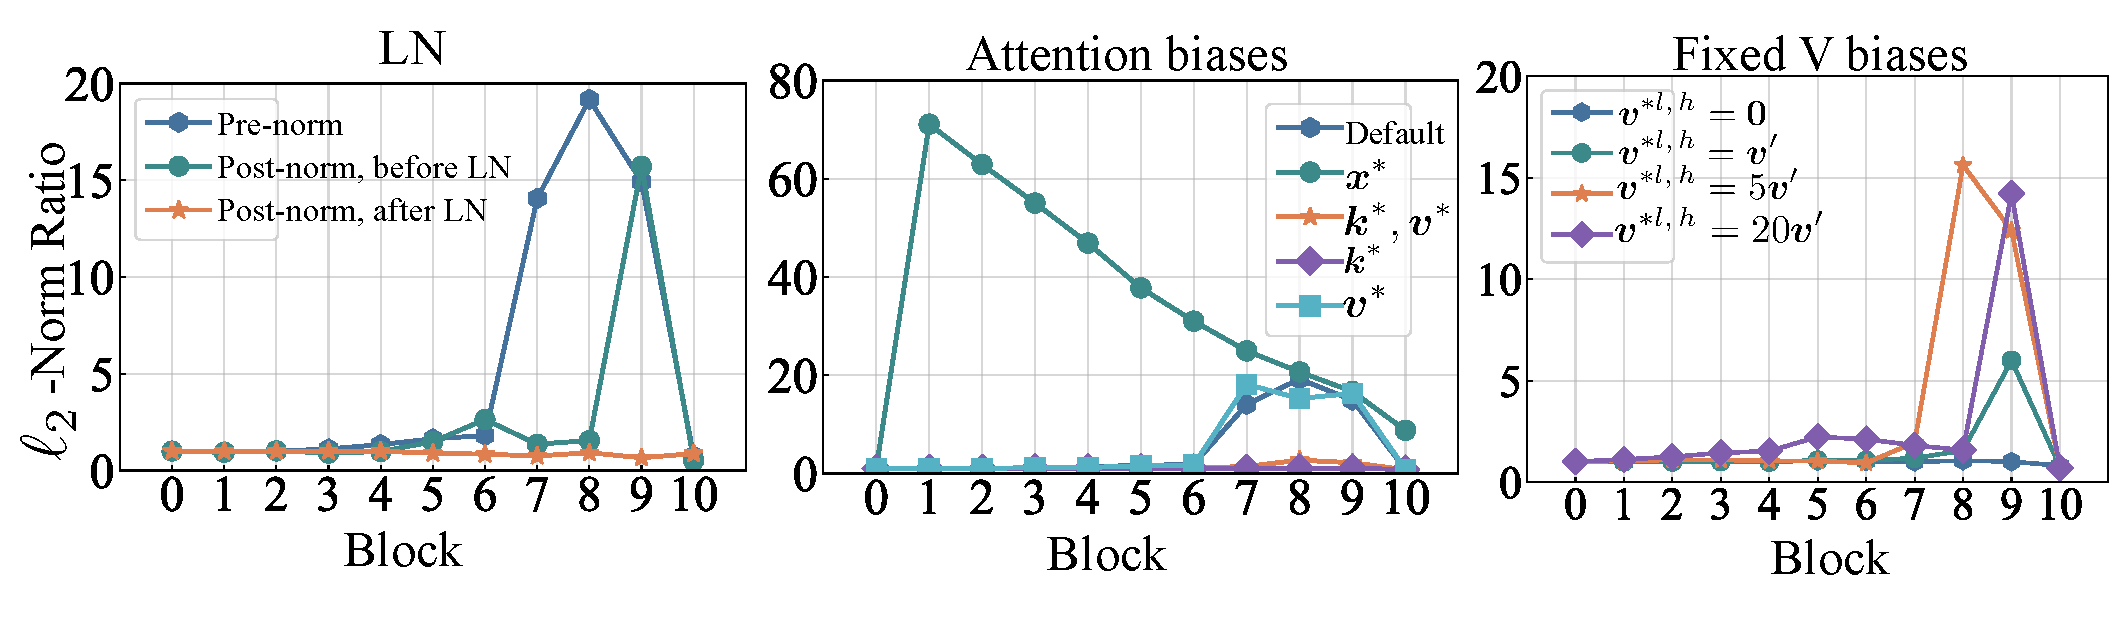
\includegraphics[width=\textwidth]{figures/massive_activations_bias.pdf}
\vspace{-0.85cm}
\caption{$\ell_2$-norm ratio of $\boldsymbol{h}_1^l$ and mean of $\boldsymbol{h}_{t\neq 0}^l$. (\emph{Left}) Massive activations exist not in hidden states in post-norm LMs, but in the features before LN. (\emph{Middle}) LMs with KV biases or K biases have no massive activations, while LMs with a learnable sink token or V biases have massive activations. (\emph{Right}) Massive activations emerge when increasing the $\ell_2$-norm of fixed $\boldsymbol{v}^{*l\textrm{,}\,h}$ for the setup of K biases.\looseness=-1 
}
\vspace{-0.35cm}
\label{massive_activations}
\end{figure}


% \begin{figure}[t]
% \centering
% % \subfigure[]{\includegraphics[width=0.45\textwidth]{figures/domains_metric1.pdf}}
% \begin{subfigure}[t]{0.64\textwidth}
%     \centering
%     \includegraphics[width=\textwidth]{figures/post-norm.pdf}
% \end{subfigure}
% \hfill
% \begin{subfigure}[t]{0.32\textwidth}
%     \centering
%     % \includegraphics[width=\textwidth]{figures/tinyllama_loss.pdf}
% \end{subfigure}
% \vspace{-0.3cm}
% \caption{(\textit{Left}) From pre-norm transformer block to post-norm transformer block. (\textit{Right}) 
% }
% \label{norm}
% \end{figure}

\begin{table}[t]
\vspace{-1.1cm}
\caption{With comparable performance, LMs with sink token, KV biases, and K biases could shift attention sink from the first token to key biases' position. Value biases cannot affect attention sink.}
\vspace{-.4cm}
\begin{center}
\begin{tabular}{l|ccc}
\toprule
 Attention in each head  &  $\textrm{Sink}_{*}^{\epsilon}$(\%) &  $\textrm{Sink}_1^{\epsilon}$(\%) &valid loss \\
\midrule
 $\textrm{Softmax}\left(\frac{1}{\sqrt{d_h}}\boldsymbol{Q}^{l\textrm{,}h}{\boldsymbol{K}^{l\textrm{,}h}}^\top+ \boldsymbol{M}\right)\boldsymbol{V}^{l\textrm{,}h}$ & - & 18.18 & 3.73 \\
 $\textrm{Softmax}\left(\frac{1}{\sqrt{d_h}}\begin{bmatrix}
    \boldsymbol{q}^{*l,h} \\
        \boldsymbol{Q}^{l,h}
    \end{bmatrix}\begin{bmatrix}
       {\boldsymbol{k}^{*l\textrm{,}h}}^\top & {\boldsymbol{K}^{l\textrm{,}h}}^\top
    \end{bmatrix}+ \boldsymbol{M}\right)\begin{bmatrix}
    \boldsymbol{v}^{*l\textrm{,}h} \\
    \boldsymbol{V}^{l\textrm{,}h}
\end{bmatrix}$ & 74.12 & \,\,\,0.00 &  3.72\\
 $\textrm{Softmax}\left(\frac{1}{\sqrt{d_h}}\boldsymbol{Q}^{l\textrm{,}h}\begin{bmatrix}
       {\boldsymbol{k}^{*l\textrm{,}h}}^\top & {\boldsymbol{K}^{l\textrm{,}h}}^\top
    \end{bmatrix}+ \boldsymbol{M}\right)\begin{bmatrix}
    \boldsymbol{v}^{*l\textrm{,}h} \\
    \boldsymbol{V}^{l\textrm{,}h}
\end{bmatrix}$ & 72.76 & \,\,\,0.04 & 3.72\\
 $\textrm{Softmax}\left(\frac{1}{\sqrt{d_h}}\boldsymbol{Q}^{l\textrm{,}h}\begin{bmatrix}
       {\boldsymbol{k}^{*l\textrm{,}h}}^\top & {\boldsymbol{K}^{l\textrm{,}h}}^\top
    \end{bmatrix}+ \boldsymbol{M}\right)\begin{bmatrix}
    \boldsymbol{0} \\
    \boldsymbol{V}^{l\textrm{,}h}
\end{bmatrix}$ & 73.34 & \,\,\,0.00 & 3.72 \\
 $\textrm{Softmax}\left(\frac{1}{\sqrt{d_h}}\boldsymbol{Q}^{l\textrm{,}h}{\boldsymbol{K}^{l\textrm{,}h}}^\top+ \boldsymbol{M}\right)\boldsymbol{V}^{l\textrm{,}h}+\boldsymbol{v}^{*l\textrm{,}h}$ & - & 17.53 & 3.73\\
\bottomrule
\end{tabular}
\end{center}
\vspace{-.2cm}
\label{bias}
\end{table}

\vspace{-0.2cm}
\subsection{Attention biases}
\vspace{-0.2cm}
\textbf{Learnable biases in attention.} In Section~\ref{section3_1}, we have shown that the first token acts as a bias: its key $\boldsymbol{k}_1^{l\textrm{,}\,h}$ is distributed in a different manifold and its value $\boldsymbol{v}_1^{l\textrm{,}\,h}$ has small $\ell_2$ norm. \citet{xiao2023efficient} considered a learnable sink token in each chunk before the input tokens during LM pre-training. As this token is fixed in the first token, this could be considered as implicitly introducing biases $\boldsymbol{k}^{*l,h}$, $\boldsymbol{v}^{*l,h}$, $\boldsymbol{q}^{*l,h}$ in attention, as shown in the second row in Table~\ref{bias}. These biases are the MLP output of $\boldsymbol{x}^*\boldsymbol{W}_E$. \citet{sun2024massive} directly introducing $\boldsymbol{k}^{*l,h}$ and $\boldsymbol{v}^{*l,h}$ as learnable parameters in attention (\emph{KV biases}). They found that this design could alleviate the massive activations. Considering the important role of $\boldsymbol{k}^{*l,h}$ and small $\ell_2$-norm of $\boldsymbol{v}^{*l,h}$ , we propose introducing only the key biases  $\boldsymbol{k}^{*l,h}$ and fix value biases $\boldsymbol{v}^{*l,h}=\boldsymbol{0}$ (\emph{K biases}). As a control, we also consider only adding value biases (\emph{V biases}). The formulations of all these attention designs are shown in Table~\ref{bias}.\looseness=-1

% As a result, attention sink appears on this learnable token $\boldsymbol{x}^*$ instead of the actual first token $\boldsymbol{x}_1$.


% \textbf{Explicit biases in attention.} \citet{sun2024massive} directly introducing $\boldsymbol{k}^{*l,h}$ and $\boldsymbol{v}^{*l,h}$ as learnable parameters in attention (\emph{KV biases}). They found that this design could alleviate the massive activations. Considering the important role of $\boldsymbol{k}^{*l,h}$ and small $\ell_2$-norm of $\boldsymbol{v}^{*l,h}$ , we propose introducing only the key biases  $\boldsymbol{k}^{*l,h}$ and fix value biases $\boldsymbol{v}^{*l,h}=\boldsymbol{0}$ (\emph{K biases}). As a control, we also consider only adding value biases (\emph{V biases}). The formulations of all these attention designs are shown in Table~\ref{bias}.\looseness=-1



% From Figure~\ref{massive}(\emph{Upper}), we observe that the $\ell_2$-norm of values for the first token is significantly smaller than the mean of other tokens. This motivates us to hypothesize that the first token plays a role in storing extra attention weights with little semantic information. To verify this hypothesize, as present in Table~\ref{bias}, we pre-train a series of models with the following setups: (i) default setup; (ii) learnable sink token following \citet{xiao2023efficient} (iii) KV biases (learnable $\boldsymbol{k}^{*l\textrm{,}h}$ and $\boldsymbol{v}^{*l\textrm{,}h}$); (iv) K biases (learnable $\boldsymbol{k}^{*l\textrm{,}h}$ and fixed $\boldsymbol{v}^{*l\textrm{,}h}=\boldsymbol{0}$); (v) V biases (fixed $\boldsymbol{k}^{*l\textrm{,}h}=\boldsymbol{0}$ and learnable $\boldsymbol{v}^{*l\textrm{,}h}$). 


% As the computation of attentions scores for $\boldsymbol{x}_{1\leq t\leq T}$ only requires the participation of $\boldsymbol{k}^{*l,h}$ and $\boldsymbol{v}^{*l,h}$ without $\boldsymbol{q}^{*l,h}$. 


% Although the focus in \citet{sun2024massive} is to use the above kv biases to alleviate massive activations, we find that attention sink also shifts from $\boldsymbol{x}_1$ to the location of this newly added $\boldsymbol{k}^{*l,h}$. 


% \begin{bmatrix}
%     \boldsymbol{q}^{*l,h} \\
%         \boldsymbol{Q}^{l,h}
%     \end{bmatrix}



% \begin{align}
%     \boldsymbol{A}_t^{l,h}&= \textrm{Softmax}\left(\frac{\begin{bmatrix}
%     <\boldsymbol{q}_t^{l,h}, \boldsymbol{k}^{*l,h}>& <\boldsymbol{q}_t^{l,h}, \boldsymbol{k}_1^{l,h}>& ...& <\boldsymbol{q}_t^{l,h}, \boldsymbol{k}_t^{l,h}>
%     \end{bmatrix}}{\sqrt{d_h}}\right)\textrm{,}\\
% \boldsymbol{O}^l&=\boldsymbol{W}_{O}^l\textrm{Concat}\left(\boldsymbol{A}^{l,1} \begin{bmatrix}
% \boldsymbol{v}^{*l,1} \\
% \boldsymbol{V}^{l,1} 
% \end{bmatrix},..., \boldsymbol{A}^{l,h}\begin{bmatrix}
% \boldsymbol{v}^{*l,h} \\
% \boldsymbol{V}^{l,h} 
% \end{bmatrix}, ...,\boldsymbol{A}^{l,H}\begin{bmatrix}
% \boldsymbol{v}^{*l,H} \\
% \boldsymbol{V}^{l,H} 
% \end{bmatrix}\right)\textrm{.}
% \end{align}





% \citet{sun2024massive} claimed that LLMs use massive activations to concentrate attention weights on specific tokens, resulting in attention sinks. Our observations show that the first token has massive activations, correlating to the initial token attention sink. After further investigation, we find that the L2 norms of values for the first token are significantly lower than that for other tokens in most layers. We hypothesize that \textbf{LLMs need registers which could save extra attention weights but have no semantic information}.  



% \begin{equation}
%     \boldsymbol{A}^{l\textrm{,}h}= \textrm{Softmax}\left(\frac{\boldsymbol{Q}^{l\textrm{,}h}
%   {\boldsymbol{K}^{l\textrm{,}h}}^T}{\sqrt{d_h}}+ \boldsymbol{M}'\right)\textrm{,}\,\,\,\,
% \boldsymbol{O}^l=\textrm{Concat}_{h=1}^H\left(\boldsymbol{A}^{l\textrm{,}h}
%     \boldsymbol{V}^{l\textrm{,}h}+\boldsymbol{v}^{*l\textrm{,}h}\right)\boldsymbol{W}_{O}^l\textrm{.}
% \end{equation}





% \begin{equation}
%     \boldsymbol{A}^{l\textrm{,}h}= \textrm{Softmax}\left(\frac{\boldsymbol{Q}^{l\textrm{,}h}{\boldsymbol{K}^{l\textrm{,}h}}^T}{\sqrt{d_h}}+ \boldsymbol{M}\right)\textrm{,}\,\,\,\,
% \boldsymbol{O}^l=\textrm{Concat}_{h=1}^H\left(\boldsymbol{A}^{l\textrm{,}h}\boldsymbol{V}^{l\textrm{,}h}\right)\boldsymbol{W}_{O}^l\textrm{.}
% \end{equation}


% \begin{equation}
%     \boldsymbol{A}^{l,h}= \textrm{Softmax}\left(\frac{\boldsymbol{Q}^{l\textrm{,}h}\begin{bmatrix}
%        {\boldsymbol{k}^{*l\textrm{,}h}}^T & {\boldsymbol{K}^{l\textrm{,}h}}^T
%     \end{bmatrix}}{\sqrt{d_h}}+ \boldsymbol{M}'\right)\textrm{,}\,\,\,\,
% \boldsymbol{O}^l=\textrm{Concat}_{h=1}^H\left(\boldsymbol{A}^{l\textrm{,}h}\begin{bmatrix}
%     \boldsymbol{v}^{*l\textrm{,}h} \\
%     \boldsymbol{V}^{l\textrm{,}h}
% \end{bmatrix}\right)\boldsymbol{W}_{O}^l\textrm{.}
% \end{equation}







% (iii) learnable $\boldsymbol{k}^{*l}$ and $\boldsymbol{v}^{*l}$, all heads in each layer share the same bias; (iv) learnable $\boldsymbol{k}^{*l,h}$ and set $\boldsymbol{v}^{*l,h}=\boldsymbol{0}$;  (v) learnable $\boldsymbol{k}^{*l}$ and set $\boldsymbol{v}^{*l}=\boldsymbol{0}$, all heads in each layer share the same bias; (vi) learnable $\boldsymbol{v}^{*l,h}$ and set $\boldsymbol{k}^{*l,h}=\boldsymbol{0}$, which is equivalent to the following formulas

% \begin{align}
%     \boldsymbol{A}_t^{l,h}&= \textrm{Softmax}\left(\frac{\begin{bmatrix} <\boldsymbol{q}_t^{l,h}, \boldsymbol{k}_1^{l,h}>& <\boldsymbol{q}_t^{l,h}, \boldsymbol{k}_2^{l,h}>& ...& <\boldsymbol{q}_t^{l,h}, \boldsymbol{k}_t^{l,h}>
%     \end{bmatrix}}{\sqrt{d_h}}\right)\textrm{,}\\
% \boldsymbol{O}^l&=\boldsymbol{W}_{O}^l\textrm{Concat}\left(\boldsymbol{A}^{l,1}\boldsymbol{V}^{l,1}+\boldsymbol{v}^{*l,1},..., \boldsymbol{A}^{l,h}\boldsymbol{V}^{l,h}+\boldsymbol{v}^{*l,h}, ...,\boldsymbol{A}^{l,H}\boldsymbol{V}^{l,H}+\boldsymbol{v}^{*l,H}\right)\textrm{.}
% \end{align}





% Afterwards, we observe the L2 norm of hidden states to investigate whether there are massive activations. 




% \begin{table}[htbp]
% \begin{center}
% \begin{tabular}{l|cccc}
% \toprule
% $\boldsymbol{k}^{*l\textrm{,}h}$ & no  & learnable  & learnable & fixed as $\boldsymbol{0}$ \\
% $\boldsymbol{v}^{*l\textrm{,}h}$ & no  & learnable & fixed as $\boldsymbol{0}$ & learnable \\
% \midrule
% $\alpha$ (\%) for $\boldsymbol{k}^*$ & - & 75.70 & 76.87 & - \\
% $\alpha$ (\%) for $\boldsymbol{k}_1$ & 21.30 & 0.26 & 0.01 & 21.65 \\

% \midrule
% $\beta$ for $\boldsymbol{k}^*$ & - &  10.83 & 11.64 & - \\
% $\beta$ for $\boldsymbol{k}_1$ & 3.52 & 0.64 & 0.35  & 3.40 \\
% \midrule
% Valid loss & 3.73 & 3.72 &  3.72 & 3.73\\
% \bottomrule
% \end{tabular}
% \end{center}
% \vspace{-.2cm}
% \caption{Comparisons among different setups of (i), (ii), (iii), and (iv).}
% \vspace{-.2cm}
% \label{k0}
% \end{table}


\textbf{LMs need key biases.} After evaluating the LMs with setups in Table~\ref{bias}, we first observe that these LMs have comparable model performance. Moreover, as long as there are key biases $\boldsymbol{k}^{*l\textrm{,}\,h}$, attention sink disappears on the first token but on the biases. From the setup of K biases, we reaffirm that the sink token acts as key biases, storing extra attention scores, which could be completely non-informative and not contribute to the value computation. It is worth mentioning that the introduced learnable sink token, KV biases, and V biases become part of model parameters in LMs. Removing them will lead to no attention sink in the first position, but a significant drop in model performance. In Figure~\ref{massive_activations}(\emph{Middle}),  we also find that the LM with a learnable sink token has massive activations in $\boldsymbol{x}^*$. While LMs with KV biases and K biases have no massive activations.\looseness=-1

% Our experiments provide a new perspective for KV cache optimization. One may consider only storing the keys of sink tokens and paying more attention to the values of other tokens.


\begin{table}[t]
\vspace{-0.2cm}
\caption{Larger $\ell_2$-norm of fixed $\boldsymbol{v}^{*l\textrm{,}h}$ results in LMs allocating more attention on $\boldsymbol{x}_1$ instead of $\boldsymbol{k}^{*l\textrm{,}h}$.\looseness=-1}
\vspace{-.4cm}
\begin{center}
\begin{tabular}{l|ccccccc}
\toprule
$\boldsymbol{v}^{*l,h}$ & $\boldsymbol{0}$ & $\boldsymbol{v}'$ & 5$\boldsymbol{v}'$ & 20$\boldsymbol{v}'$ & $\boldsymbol{v}''$ & 5$\boldsymbol{v}''$  & 20$\boldsymbol{v}''$  \\
\midrule
$\textrm{Sink}_{*}^{\epsilon}$(\%) & 73.34 & 70.03 & 44.43 & \,\,\,1.51 & 69.74 & 27.99 &  \,\,\,0.00 \\
$\textrm{Sink}_{1}^{\epsilon}$(\%) & \,\,\,0.00 &  \,\,\,0.06 & \,\,\,3.71 & 25.88 & \,\,\,2.15 & \,\,\,5.93 & 11.21 \\
valid loss & \,\,\,3.72 & \,\,\,3.72 & \,\,\,3.72 & \,\,\,3.71 & \,\,\,3.72 & \,\,\,3.72 & \,\,\,3.73 \\
\bottomrule
\end{tabular}
\end{center}
\vspace{-.4cm}
\label{v_norm}
\end{table}

% \begin{table}[t]
% \vspace{-0.2cm}
% \caption{Larger $\ell_2$-norm of fixed $\boldsymbol{v}^{*l\textrm{,}h}$ results in LMs allocating more attention on $\boldsymbol{x}_1$ instead of $\boldsymbol{k}^{*l\textrm{,}h}$.}
% \vspace{-.4cm}
% \begin{center}
% \begin{tabular}{l|ccccccc}
% \toprule
% $\boldsymbol{v}^{*l,h}$ & $\boldsymbol{0}$ & $\boldsymbol{v}'$ & 5$\boldsymbol{v}'$ & 20$\boldsymbol{v}'$ & $\boldsymbol{v}''$ & 5$\boldsymbol{v}''$  & 20$\boldsymbol{v}''$  \\
% \midrule
% $\textrm{Sink}_{*}^{\epsilon}$(\%) & 73.34 & 70.03 & 44.43 & \,\,\,1.51 & 69.74 & 27.99 &  \,\,\,0.00 \\
% $\textrm{Sink}_{1}^{\epsilon}$(\%) & \,\,\,0.00 &  \,\,\,0.06 & \,\,\,3.71 & 25.88 & \,\,\,2.15 & \,\,\,5.93 & 11.21 \\
% valid loss & \,\,\,3.72 & \,\,\,3.72 & \,\,\,3.72 & \,\,\,3.71 & \,\,\,3.72 & \,\,\,3.72 & \,\,\,3.73 \\
% \bottomrule
% \end{tabular}
% \end{center}
% \vspace{-.4cm}
% \label{low_rank}
% \end{table}

\textbf{Beyond all zeros in V biases.} In the setup of K biases, we fix $\boldsymbol{v}^{*l,h}=\boldsymbol{0}$. We wonder whether the fixed values of $\boldsymbol{v}^{*l,h}$ could affect the attention sink. We consider, $\boldsymbol{v}^{*l,h}=m\boldsymbol{v}'$ or $\boldsymbol{v}^{*l,h}=m\boldsymbol{v}''$, where $m$ is the controllable $\ell_2$ norm and $\boldsymbol{v}'=[1,0,0,..,0]$ and $\boldsymbol{v}''=[1,1,1,..,1]/ \sqrt{d_h}$. As shown in Table~\ref{v_norm}, with larger $\ell_2$-norm of $\boldsymbol{v}^{*l,h}$, attention sink shifts from $\boldsymbol{k}^{*l,h}$ to the first token. Intuitively, it is difficult for LMs to remove the effects of $\boldsymbol{v}^{*l,h}$ with larger $\ell_2$-norm in model predictions. Then they opt to optimize the keys and values of the first token to save extra attention. 

\textbf{Design space of biases.} In Table~\ref{multi_head}(\emph{Right}), the LM with head-sharing KV biases tends to shift the sink from $\boldsymbol{k}^{*l,h}$ back to the first token. While the one with head-sharing K biases is less affected. In Table~\ref{k_low_rank}, even with small learnable dimensions for key biases, they can still absorb large attention.\looseness=-1

% explore whether different heads in each block can share the same parameters for KV biases. Results in Table~\ref{multi_head}(\emph{Right}) show that the LM with KV biases tends to shift the attention sink from $\boldsymbol{k}^{*l,h}$ back to the first token. While the LM with K biases is less affected.\looseness=-1



% \begin{figure}[t]
% \centering
% % \subfigure[]{\includegraphics[width=0.45\textwidth]{figures/domains_metric1.pdf}}
% \begin{subfigure}[t]{0.48\textwidth}
%     \centering
%     \includegraphics[width=\textwidth]{figures/massive_activations.pdf}
% \end{subfigure}
% \hfill
% \begin{subfigure}[t]{0.48\textwidth}
%     \centering
%     % \includegraphics[width=\textwidth]{figures/massive_activations.pdf}
% \end{subfigure}
% \vspace{-0.3cm}
% \caption{L2 norm of (\textit{Left}) the hidden states and (\textit{Right}) the values for Llama-2-7B model.
% }
% \label{lengths}
% \end{figure}




% From our experiments, we hypothesize that the newly introduced $\boldsymbol{k}^{l\textrm{,}h}$ or the sink token increases the degree of freedom when computing the attention. To validate this, we replace softmax attention with sigmoid attention. A concurrent work~\citep{ramapuram2024theory} propose sigmoid attention.  


\vspace{-0.2cm}
\subsection{Attention operation}
\vspace{-0.2cm}
\textbf{General formulation of attention.} In the last section, we realize that LMs need key biases to save extra attention. This motivates us to explore whether such a property is related to the dependence among attention scores due to the softmax operation. First, the attention output for the $i$-th token can be generalized as: $\boldsymbol{v}_i^{\dagger}=\left(\sum_{j'=1}^i\textrm{sim}(\varphi(\boldsymbol{q}_i)\textrm{,}\,\varphi(\boldsymbol{k}_{j'}))\right)^{-1}\sum_{j=1}^i\textrm{sim}(\varphi(\boldsymbol{q}_i)\textrm{,}\,\varphi(\boldsymbol{k}_j))\boldsymbol{v}_j=\boldsymbol{Z}_i^{-1}\sum_{j=1}^i\textrm{sim}(\varphi(\boldsymbol{q}_i)\textrm{,}\,\varphi(\boldsymbol{k}_j))\boldsymbol{v}_j$,
% \looseness=-1
% \begin{equation}
% \boldsymbol{v}_i'=\sum_{j=1}^i\frac{\textrm{sim}(\varphi(\boldsymbol{q}_i)\textrm{,}\,\varphi(\boldsymbol{k}_j))}{\sum_{j'=1}^i\textrm{sim}(\varphi(\boldsymbol{q}_i)\textrm{,}\,\varphi(\boldsymbol{k}_{j'}))}\boldsymbol{v}_j=\sum_{j=1}^i\frac{\textrm{sim}(\varphi(\boldsymbol{q}_i)\textrm{,}\,\varphi(\boldsymbol{k}_j))}{\boldsymbol{Z}_i}\boldsymbol{v}_j\textrm{,}
% \end{equation}
where we omit the PE, and block/head indexes for simplicity. $\boldsymbol{Z}_i$ is a normalization term and $\varphi(\cdot)$ is a kernel function. Normally, $\boldsymbol{Z}_i=\sum_{j'=1}^i\textrm{sim}(\varphi(\boldsymbol{q}_i)\textrm{,}\,\varphi(\boldsymbol{k}_j))$. For softmax attention, $\varphi(\cdot)$ is an identity kernel and $\textrm{sim}(\boldsymbol{q}_i\textrm{,}\,\boldsymbol{k}_j)=\textrm{exp}(\boldsymbol{q}_i\boldsymbol{k}_j^\top/\sqrt{d_h})$.

% It is noted that the attention output for $i$-th token $\boldsymbol{v}_i'$ only considers keys and values of previous tokens due to the casual mask. 


\textbf{Normalization.} In Table~\ref{reweight}(\emph{Left}) and Figure~\ref{appendix_normalizer}, we show that modifying normalization may result in less obvious attention sink but does not stop its emergence. So we consider removing the normalization. Since the exponential function in softmax tends to explode without normalization, we replace it with sigmoid or elu plus one. When evaluating the attention sink, we compute the \textit{proxy} attention scores by using the term $\boldsymbol{Z}_i=\sum_{j'=1}^i\textrm{sim}(\varphi(\boldsymbol{q}_i)\textrm{,}\,\varphi(\boldsymbol{k}_{j'}))$ for attention sink metric $\textrm{Sink}_1^{\epsilon}$. As shown in Table~\ref{operation}, without normalization, LMs still have comparable validation loss but no attention sink. With normalization, attention sink also emerges in LMs with sigmoid attention.\looseness=-1


% $\boldsymbol{Z}_i=[\sum_{j'=1}^i\textrm{sim}(\varphi(\boldsymbol{q}_i)\textrm{,}\,\varphi(\boldsymbol{k}_{j'}))^p]^{\frac{1}{p}}$

% \begin{table}[t]
% \vspace{-1.cm}
% \caption{Normalization and selections of kernels in attention significantly affect the emergence of the attention sink. We use ``*'' to mark that the metric $\textrm{Sink}_1^{\epsilon}$ is computed by proxy attention scores.}
% %We use ``-'' to represent the training failure under the setup.
% \vspace{-.4cm}
% \begin{center}
% \begin{tabular}{l|l|cc}
% \toprule
%   $\textrm{sim}(\varphi(\boldsymbol{q}_i)\textrm{,}\,\varphi(\boldsymbol{k}_j))$ & $\boldsymbol{Z}_i$ & $\textrm{Sink}_1^{\epsilon}$(\%) & loss \\
% \midrule
%  $\textrm{exp}(\boldsymbol{q}_i^T\boldsymbol{k}_j/\sqrt{d_h})$ & $\sum_{j'=1}^i \textrm{exp}(\boldsymbol{q}_i\boldsymbol{k}_{j'}^T/\sqrt{d_h})$ & 18.18 & 3.73 \\
%  $\textrm{sigmoid}(\boldsymbol{q}_i\boldsymbol{k}_j^T/\sqrt{d_h})$ & $1$ & \,\,\,\,\,\,0.44$^*$ &  3.70 \\
% $\textrm{sigmoid}(\boldsymbol{q}_i\boldsymbol{k}_j^T/\sqrt{d_h})$ & $\sum_{j'=1}^i \textrm{sigmoid}(\boldsymbol{q}_i\boldsymbol{k}_{j'}^T/\sqrt{d_h})$ & 30.24 & 3.74 \\
%  $\textrm{elu}(\boldsymbol{q}_i\boldsymbol{k}_j^T/\sqrt{d_h})+1$ & $1$ & \,\,\,\,\,\,0.80$^*$ &  3.69 \\ 
%  % $\textrm{elu}(\frac{\boldsymbol{q}_i\boldsymbol{k}_{j}^T}{\sqrt{d_h}})+1$ & $\sum_{j'=1}^i \textrm{elu}(\frac{\boldsymbol{q}_i\boldsymbol{k}_{j'}^T}{\sqrt{d_h}})+1$ & - & - \\ 
%  \midrule
% $(\textrm{elu}(\boldsymbol{q}_i)+1)(\textrm{elu}(\boldsymbol{k}_j)+1)^T$ & $\sum_{j'=1}^i(\textrm{elu}(\boldsymbol{q}_i)+1)(\textrm{elu}(\boldsymbol{k}_{j'})+1)^T$ & \,\,\,53.65$^*$ & 4.19\\ 
% % $\frac{(\textrm{elu}(\boldsymbol{q}_i)+1)(\textrm{elu}(\boldsymbol{k}_j)+1)^T}{\sqrt{d_h}}$ & $1$ & -  & - \\ 
% % $\frac{\boldsymbol{q}_i\boldsymbol{k}_{j}^T}{\sqrt{d_h}}$ &  $\textrm{max}\left(\left|\sum_{j'=1}^i\frac{\boldsymbol{q}_i\boldsymbol{k}_{j'}^T}{\sqrt{d_h}}\right|\textrm{,}\,1\right)$ & - &  -\\
% $\boldsymbol{q}_i\boldsymbol{k}_{j}^T/\sqrt{d_h}$ & $1$ & \,\,\,\,\,0.00$^*$ & 3.99 \\
% $\textrm{mlp}(\boldsymbol{q}_i)\textrm{mlp}(\boldsymbol{k}_j)^T/\sqrt{d_h}$ &  $\textrm{max}(|\sum_{j'=1}^i\textrm{mlp}(\boldsymbol{q}_i)\textrm{mlp}(\boldsymbol{k}_{j'})^T/\sqrt{d_h}|\textrm{,}\,1)$ & \,\,\,\,\,0.19$^*$ &  3.85\\
% $\textrm{mlp}(\boldsymbol{q}_i)\textrm{mlp}(\boldsymbol{k}_j)^T/\sqrt{d_h}$ & $1$ & \,\,\,\,\,0.74$^*$ & 3.91 \\
% \bottomrule
% \end{tabular}
% \end{center}
% \vspace{-.5cm}
% \label{operation}
% \end{table}

\begin{table}[t]
\vspace{-1.1cm}
\caption{Normalization and selections of kernels in attention significantly affect the emergence of the attention sink. We use ``*'' to mark that the metric $\textrm{Sink}_1^{\epsilon}$ is computed by proxy attention scores.}
\vspace{-.2cm}
\begin{center}
\begin{tabular}{l|l|cc}
\toprule
  $\textrm{sim}(\varphi(\boldsymbol{q}_i)\textrm{,}\,\varphi(\boldsymbol{k}_j))$ & $\boldsymbol{Z}_i$ & $\textrm{Sink}_1^{\epsilon}$(\%) & valid loss \\
\midrule
 $\textrm{exp}(\frac{\boldsymbol{q}_i\boldsymbol{k}_j^\top}{\sqrt{d_h}})$ & $\sum_{j'=1}^i \textrm{exp}(\frac{\boldsymbol{q}_i\boldsymbol{k}_{j'}^\top}{\sqrt{d_h}})$ & 18.18 & 3.73 \\
 $\textrm{sigmoid}(\frac{\boldsymbol{q}_i\boldsymbol{k}_j^\top}{\sqrt{d_h}})$ & $1$ & \,\,\,\,\,\,0.44$^*$ &  3.70 \\
$\textrm{sigmoid}(\frac{\boldsymbol{q}_i\boldsymbol{k}_j^\top}{\sqrt{d_h}})$ & $\sum_{j'=1}^i \textrm{sigmoid}(\frac{\boldsymbol{q}_i\boldsymbol{k}_{j'}^\top}{\sqrt{d_h}})$ & 30.24 & 3.74 \\
 $\textrm{elu}(\frac{\boldsymbol{q}_i\boldsymbol{k}_j^\top}{\sqrt{d_h}})+1$ & $1$ & \,\,\,\,\,\,0.80$^*$ &  3.69 \\ 
 % $\textrm{elu}(\frac{\boldsymbol{q}_i\boldsymbol{k}_{j}^T}{\sqrt{d_h}})+1$ & $\sum_{j'=1}^i \textrm{elu}(\frac{\boldsymbol{q}_i\boldsymbol{k}_{j'}^T}{\sqrt{d_h}})+1$ & - & - \\ 
 \midrule
$\frac{(\textrm{elu}(\boldsymbol{q}_i)+1)(\textrm{elu}(\boldsymbol{k}_j)+1)^\top}{\sqrt{d_h}}$ & $\sum_{j'=1}^i\frac{(\textrm{elu}(\boldsymbol{q}_i)+1)(\textrm{elu}(\boldsymbol{k}_{j'})+1)^\top}{\sqrt{d_h}}$ & \,\,\,53.65$^*$ & 4.19\\ 
% $\frac{(\textrm{elu}(\boldsymbol{q}_i)+1)(\textrm{elu}(\boldsymbol{k}_j)+1)^T}{\sqrt{d_h}}$ & $1$ & -  & - \\ 
% $\frac{\boldsymbol{q}_i\boldsymbol{k}_{j}^T}{\sqrt{d_h}}$ &  $\textrm{max}\left(\left|\sum_{j'=1}^i\frac{\boldsymbol{q}_i\boldsymbol{k}_{j'}^T}{\sqrt{d_h}}\right|\textrm{,}\,1\right)$ & - &  -\\
$\frac{\boldsymbol{q}_i\boldsymbol{k}_{j}^\top}{\sqrt{d_h}}$ & $1$ & \,\,\,\,\,0.00$^*$ & 3.99 \\
$\frac{\textrm{mlp}(\boldsymbol{q}_i)\textrm{mlp}(\boldsymbol{k}_j)^\top}{\sqrt{d_h}}$ &  $\textrm{max}\left(\left|\sum_{j'=1}^i\frac{\textrm{mlp}(\boldsymbol{q}_i)\textrm{mlp}(\boldsymbol{k}_{j'})^\top}{\sqrt{d_h}}\right|\textrm{,}\,1\right)$ & \,\,\,\,\,0.19$^*$ &  3.85\\
$\frac{\textrm{mlp}(\boldsymbol{q}_i)\textrm{mlp}(\boldsymbol{k}_j)^\top}{\sqrt{d_h}}$ & $1$ & \,\,\,\,\,0.74$^*$ & 3.91 \\
\bottomrule
\end{tabular}
\end{center}
\vspace{-.2cm}
\label{operation}
\end{table}

\begin{figure}[t]
\centering
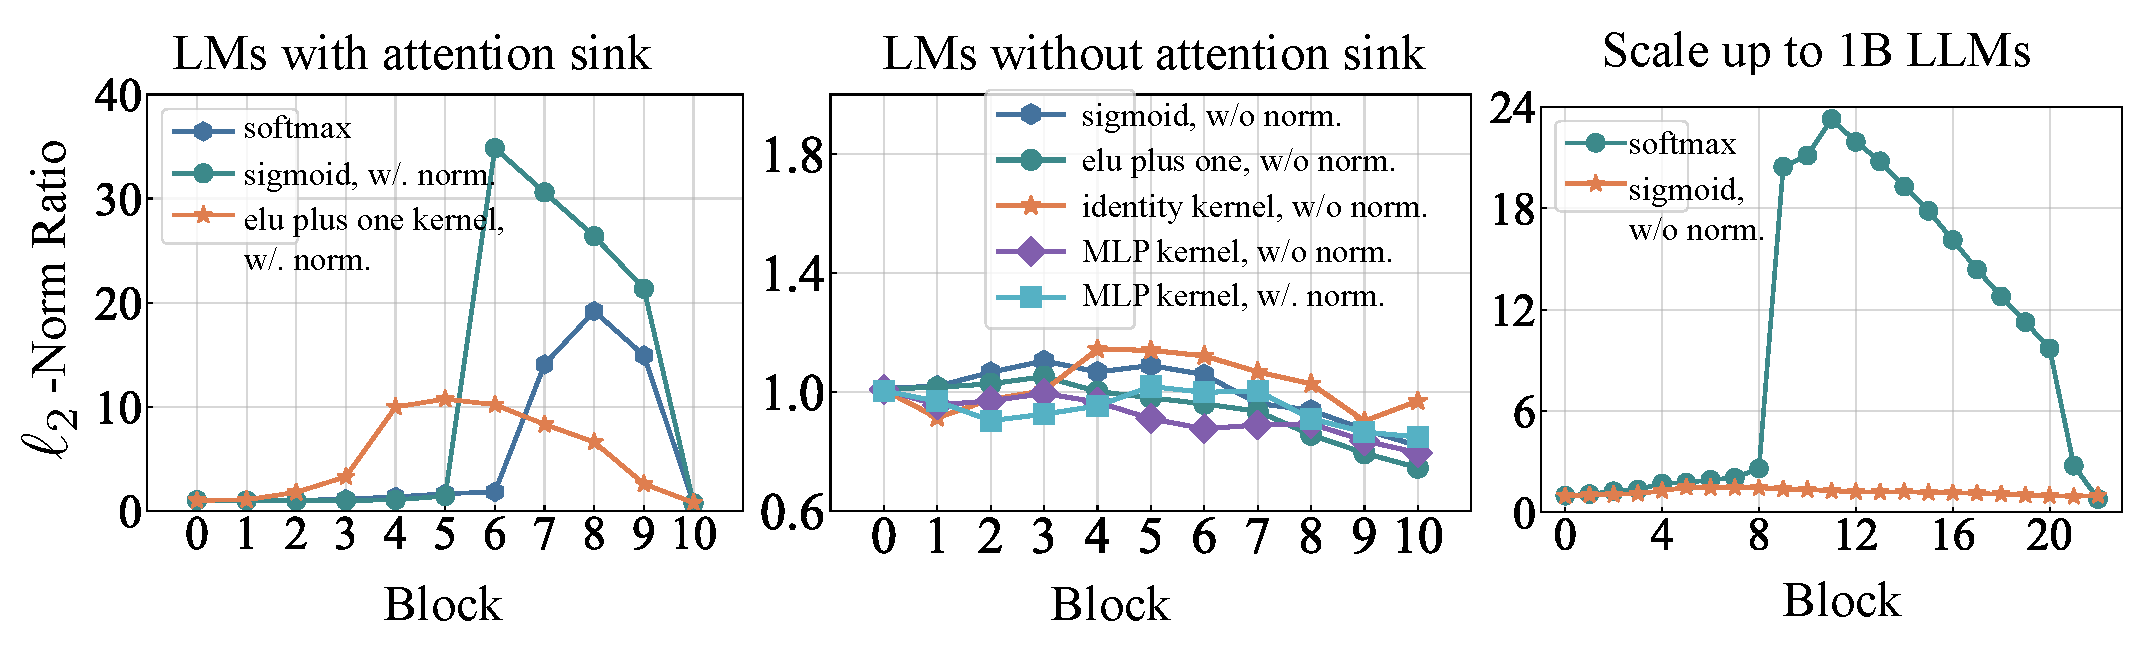
\includegraphics[width=\textwidth]{figures/massive_activations_operations.pdf}
\vspace{-0.85cm}
\caption{We visualize the $\ell_2$-norm ratio of $\boldsymbol{h}_1^l$ and mean of $\boldsymbol{h}_{t\neq 0}^l$. (\emph{Left}) Massive activations exist in LMs with attention scores that are non-negative and added up to one. (\emph{Middle}) Massive activations do not exist in LMs with independent attention scores. (\emph{Right}) When scaling the model size to 1B, LLMs with sigmoid attention (no normalization) still have no massive activations.\looseness=-1 
}
\vspace{-0.2cm}
\label{massive_activations_operation}
\end{figure}

\textbf{Kernel functions.} Motivated by linear attention~\citep{katharopoulos2020transformers}, we consider different kernel functions $\varphi(\cdot)$, including elu plus one, identity, and MLP. It is noted that  $\textrm{sim}(\varphi(\boldsymbol{q}_i)\textrm{,}\,\varphi(\boldsymbol{k}_{j'}))$ could be minus for identity and MLP kernels. This brings intrinsic difficulty for normalization during the training and calculation of $\textrm{Sink}_1^{\epsilon}$. For normalization in the training, we consider $\boldsymbol{Z}_i=\textrm{max}\big(\big|\sum_{j'=1}^i\textrm{sim}(\varphi(\boldsymbol{q}_i)\textrm{,}\,\varphi(\boldsymbol{k}_{j'}))\big|\textrm{,}\,1\big)$. When computing $\textrm{Sink}_1^{\epsilon}$, we consider the proxy attention scores $\left|\textrm{sim}(\varphi(\boldsymbol{q}_i)\textrm{,}\,\varphi(\boldsymbol{k}_j))\right|/\sum_{j'=1}^i\left|\textrm{sim}(\varphi(\boldsymbol{q}_i)\textrm{,}\,\varphi(\boldsymbol{k}_{j'}))\right|$. From Table~\ref{operation} (a full version in Table~\ref{appendix_operation}), we find that the LM with MLP kernel have no attention sink with or without normalization.\looseness=-1

\textbf{Inner dependence on attention scores.} We note that the LMs with no attention sink typically relax tokens' inner dependence on attention scores. Their attention scores during pre-training could be negative or not add up to one. This indicated that attention sink (at least partially) stems from such inner dependence. Besides the attention metric computed by proxy attention scores, we also observe that the above LMs also have no massive activations, as shown in Figure~\ref{massive_activations_operation}(\emph{Middle}). 

\textbf{Scale up to 1B parameters.} We compare model behaviors of 1B LMs with softmax attention and sigmoid attention (without normalization). Specifically, the latter achieves a validation loss of 3.10, slightly larger than the 3.07 achieved by the former. However, the attention sink metric significantly drops from 45.11\% to near zero: $\textrm{Sink}_1^{\epsilon}=\textrm{2.46\%}$ using the proxy attention scores. Meanwhile, as present in Figure~\ref{massive_activations_operation}(\emph{Right}), LLMs with sigmoid attention have no massive activations. Furthermore, they have no issues of training stability during continued supervised fine-tuning in Appendix~\ref{sft}.\looseness=-1


% \vspace{-0.1cm}
\begin{abox} % are we tired of takeaway boxes? :>
    \looseness -1 \textbf{Takeaways:} 1.~Positional embedding, FFN design, LN location, and multi-head design do not affect the emergence of attention sink. 2.~Attention sink acts more like key biases, storing extra attention and meanwhile not contributing to the value computation. 3.~When relaxing tokens' inner dependence on attention scores, attention sink does not emerge in LMs. % at test time.
\end{abox}

% Firstly, we only consider replacing the exponential function with other functions, such as sigmoid and ELU plus one. Then we also explore whether there are attention sinks in linear attention.





% \begin{table}[htbp]
% \begin{center}
% \begin{tabular}{ll|cc}
% \toprule
%   $\textrm{sim}(\boldsymbol{q}_i\textrm{,}\,\boldsymbol{k}_j)$ & $\boldsymbol{Z}_i$ & $\textrm{Sink}_1^{\epsilon}$(\%) & Valid loss \\
% \midrule
%  $\textrm{exp}(\frac{\boldsymbol{q}_i^T\boldsymbol{k}_j}{\sqrt{d_h}})$ & $\sum_{j'=1}^i \textrm{exp}(\frac{\boldsymbol{q}_i\boldsymbol{k}_{j'}^T}{\sqrt{d_h}})$ & 18.18 & 3.73 \\
%  $\textrm{sigmoid}(\frac{\boldsymbol{q}_i\boldsymbol{k}_j^T}{\sqrt{d_h}})$ & $1$ & 0.44 &  3.70 \\
% $\textrm{sigmoid}(\frac{\boldsymbol{q}_i\boldsymbol{k}_j^T}{\sqrt{d_h}})$ & $\sum_{j'=1}^i \textrm{sigmoid}(\frac{\boldsymbol{q}_i\boldsymbol{k}_{j'}^T}{\sqrt{d_h}})$ & 30.24 & 3.74 \\
%  $\textrm{elu}(\frac{\boldsymbol{q}_i\boldsymbol{k}_j^T}{\sqrt{d_h}})+1$ & $1$ & 0.80 &  3.69 \\ 
%  $\textrm{elu}(\frac{\boldsymbol{q}_i\boldsymbol{k}_{j}^T}{\sqrt{d_h}})+1$ & $\sum_{j'=1}^i \textrm{elu}(\frac{\boldsymbol{q}_i\boldsymbol{k}_{j'}^T}{\sqrt{d_h}})+1$ & 0.51 & 8.21 \\ 
%  \midrule
% $\frac{(\textrm{elu}(\boldsymbol{q}_i)+1)(\textrm{elu}(\boldsymbol{k}_j)+1)^T}{\sqrt{d_h}}$ & $\sum_{j'=1}^i\frac{(\textrm{elu}(\boldsymbol{q}_i)+1)(\textrm{elu}(\boldsymbol{k}_{j'})+1)^T}{\sqrt{d_h}}$ & 58.59 & 4.19\\ 
% $\frac{(\textrm{elu}(\boldsymbol{q}_i)+1)(\textrm{elu}(\boldsymbol{k}_j)+1)^T}{\sqrt{d_h}}$ & $1$ & 0.00  & 4.89 \\ 
% $\frac{\boldsymbol{q}_i\boldsymbol{k}_{j}^T}{\sqrt{d_h}}$ &  $\textrm{max}\left(\left|\sum_{j'=1}^i\frac{\boldsymbol{q}_i\boldsymbol{k}_{j'}^T}{\sqrt{d_h}}\right|\textrm{,}\,1\right)$ & 0.00 &  7.86\\
% $\frac{\boldsymbol{q}_i\boldsymbol{k}_{j}^T}{\sqrt{d_h}}$ & $1$ & 0.00 & 3.99 \\
% $\frac{\textrm{mlp}(\boldsymbol{q}_i)\textrm{mlp}(\boldsymbol{k}_j)^T}{\sqrt{d_h}}$ &  $\textrm{max}\left(\left|\sum_{j'=1}^i\frac{\textrm{mlp}(\boldsymbol{q}_i)\textrm{mlp}(\boldsymbol{k}_{j'})^T}{\sqrt{d_h}}\right|\textrm{,}\,1\right)$ & 0.19 &  3.85\\
% $\frac{\textrm{mlp}(\boldsymbol{q}_i)\textrm{mlp}(\boldsymbol{k}_j)^T}{\sqrt{d_h}}$ & $1$ & 0.74 & 3.91 \\
% \bottomrule
% \end{tabular}
% \end{center}
% \vspace{-.2cm}
% \caption{Replacing softmax attention with other attention operations.}
% \vspace{-.2cm}
% \label{operation}
% \end{table}




% \begin{table}[htbp]
% \begin{center}
% \begin{tabular}{l|cccc}
% \toprule
% $\varphi$  & normalization &  $\alpha_1$ & $\beta_1$ & Valid loss \\
% \midrule
% $\frac{(\textrm{elu}(\boldsymbol{q}_i)+1)(\textrm{elu}(\boldsymbol{k}_j)+1)^T}{\sqrt{d_h}}$ & $\sum_{j'=1}^i\frac{(\textrm{elu}(\boldsymbol{q}_i)+1)(\textrm{elu}(\boldsymbol{k}_{j'})+1)^T}{\sqrt{d_h}}$ & 58.59 & 7.81 & 4.19\\ 
% $\frac{(\textrm{elu}(\boldsymbol{q}_i)+1)(\textrm{elu}(\boldsymbol{k}_j)+1)^T}{\sqrt{d_h}}$ & 1 & 0.01  & 0.91 & 4.89 \\ 
% $\frac{\boldsymbol{q}_i\boldsymbol{k}_{j}^T}{\sqrt{d_h}}$ &  $\sum_{j'=1}^i\frac{\boldsymbol{q}_i\boldsymbol{k}_{j'}^T}{\sqrt{d_h}}$ & 0.00 & 1.01 & 7.86\\
% $\frac{\boldsymbol{q}_i\boldsymbol{k}_{j}^T}{\sqrt{d_h}}$ & 1 & 0.00 & 0.77 & 3.99 \\
% $\frac{\textrm{mlp}(\boldsymbol{q}_i)\textrm{mlp}(\boldsymbol{k}_j)^T}{\sqrt{d_h}}$ &  $\sum_{j'=1}^i\frac{\textrm{mlp}(\boldsymbol{q}_i)\textrm{mlp}(\boldsymbol{k}_{j'})^T}{\sqrt{d_h}}$ & 0.33 & 0.83 & 3.85\\
% $\frac{\textrm{mlp}(\boldsymbol{q}_i)\textrm{mlp}(\boldsymbol{k}_j)^T}{\sqrt{d_h}}$ & 1 & 0.94 & 0.89 & 3.91 \\
% \bottomrule
% \end{tabular}
% \end{center}
% \vspace{-.2cm}
% \caption{Replacing softmax attention with linear attention operations.}
% \vspace{-.2cm}
% \label{linear}
% \end{table}


% $\textrm{elu}(\frac{\boldsymbol{q}_i\boldsymbol{k}_j^T}{\sqrt{d_h}})+1$
% $\frac{\boldsymbol{q}_i\boldsymbol{k}_j^T}{\sqrt{d_h}}$
% $\frac{\textrm{MLP}(\boldsymbol{q}_i)\textrm{MLP}(\boldsymbol{k}_j)^T}{\sqrt{d_h}}$

% \begin{table}[htbp]
% \begin{center}
% \begin{tabular}{l|ccc}
% \toprule
%  Attention & Softmax & Sigmoid w/o normalization & Sigmoid w/. normalization \\
% \midrule
% $\alpha_1$ (\%) & 21.30 & 0.74 & 33.72 \\
% % \midrule
% $\beta_1$ & 3.52 & 0.62 & 4.30  \\
% Valid loss & 3.73 &  3.70 & 3.74  \\
% \bottomrule
% \end{tabular}
% \end{center}
% \vspace{-.2cm}
% \caption{Replacing softmax attention with sigmoid attention.}
% \vspace{-.2cm}
% \label{sigmoid}
% \end{table}


% \begin{table}[t]
% \begin{center}
% \begin{tabular}{l|cccc}
% \toprule
% Batch size & 128 & 256 & 512 & 1024 \\
% \midrule
% $\alpha_1$ (\%) & 18.30 & 19.52 & 20.94 & 21.35\\
% % \midrule
% $\beta_1$ & 3.18 & 3.16 & 3.38 & 3.27 \\
% \bottomrule
% \end{tabular}
% \end{center}
% \vspace{-.2cm}
% \caption{Batch size.}
% \vspace{-.2cm}
% \label{tbl_decay_ema}
% \end{table}


% \begin{theorem}\label{theorem2}
% Decoder-only LLMs with casual masks have the inductive bias to reduce the rank of hidden states.
% \end{theorem}

% \textbf{Data distribution.} We modify the data distribution to observe its effect on attention sink. 

% Firstly, we consider fixed tokens $p(\boldsymbol{x}_t)=\mathbb{I}(\boldsymbol{x}_t==\boldsymbol{x})$, which means the $t$-th token is fixed as $\boldsymbol{x}$, e.g. <pad> token for all training sequences. This operation is similar to \citet{xiao2023efficient}, where the authors add learnable tokens before the initial token. If we remove this token or use normal data during the inference, $\alpha_{1:4}<1.0$.

% \begin{table}[htbp]
% \begin{center}
% \begin{tabular}{l|cccc}
% \toprule
% Token position & $\boldsymbol{x}_1=$<pad> & $\boldsymbol{x}_2=$<pad> & $\boldsymbol{x}_3=$<pad> \\
% \midrule
% $\alpha_1$ (\%) & 76.04 & <1 & <1 \\
% $\alpha_2$ (\%) & <1 & 75.12 & <1 \\
% $\alpha_3$ (\%) & <1 & <1 & 76.76 \\
% $\alpha_4$ (\%) & <1 & <1 & <1 \\
% % % \midrule
% % $\beta_1$ & 3.18 & 3.16 & 3.38 & 3.27 \\
% \bottomrule
% \end{tabular}
% \end{center}
% \vspace{-.2cm}
% \caption{Fixed token.}
% \vspace{-.2cm}
% \label{tbl_decay_ema}
% \end{table}

% Secondly, we consider random tokens. If we use normal data, the results are similar.

% \begin{table}[htbp]
% \begin{center}
% \begin{tabular}{l|cccccc}
% \toprule
% Token position & $\boldsymbol{x}_1\sim\mathbb{V}$ & $\boldsymbol{x}_2\sim\mathbb{V}$  & $\boldsymbol{x}_{1,2}\sim\mathbb{V}$ &$\boldsymbol{x}_{1,2,3,4,5}\sim\mathbb{V}$ & $\boldsymbol{x}_{2,3,4,5}\sim\mathbb{V}$ & $\boldsymbol{x}_{3,4,5}\sim\mathbb{V}$\\
% \midrule
% $\alpha_1$ (\%) & 33.67 & 25.05 & 12.31 & 2.40 & 2.31 & <1\\
% $\alpha_2$ (\%) & <1 & <1 & 21.29 & 1.05 & 1.25 & <1 \\
% $\alpha_3$ (\%) & <1 & <1 & <1 & 0.89 & 1.25 & 5.78\\
% $\alpha_4$ (\%) & <1 & <1 & <1 & 0.77 & 1.20 & 6.17\\
% $\alpha_5$ (\%) & <1 & <1 & <1 & 1.24 & 1.28 & 5.32\\
% $\alpha_6$ (\%) & <1 & <1 & <1 & <1 & 0.28 & <1 \\
% % % \midrule
% % $\beta_1$ & 3.18 & 3.16 & 3.38 & 3.27 \\
% \bottomrule
% \end{tabular}
% \end{center}
% \vspace{-.2cm}
% \caption{Random token.}
% \vspace{-.2cm}
% \label{tbl_decay_ema}
% \end{table}

% We consider pre-fix language models:

% \begin{table}[htbp]
% \begin{center}
% \begin{tabular}{l|ccccc}
% \toprule
% Unmasked tokens & 2 & 3 & 4 & 5 & 10 \\
% \midrule
% $\alpha_1$ (\%) & 4.96 & 8.47 & 3.05 & 1.80 & <1\\
% $\alpha_2$ (\%) & 9.89 & 6.97 & 8.88 & 7.30 & 2.50\\
% $\alpha_3$ (\%) & 3.37 & 2.08 & 4.59 & 4.62 & 4.15\\
% $\alpha_4$ (\%) & 1.5 & <1 & 2.26 & 2.35 & 3.90\\
% $\alpha_5$ (\%) & < 1 & <1 & <1 & 1.46 & 3.73\\
% % % \midrule
% % $\beta_1$ & 3.18 & 3.16 & 3.38 & 3.27 \\
% \bottomrule
% \end{tabular}
% \end{center}
% \vspace{-.2cm}
% \caption{Prefix Large Language Models.}
% \vspace{-.2cm}
% \label{tbl_decay_ema}
% \end{table}



% \subsection{Token Asymmetry}

% \textbf{Attention casual mask.}

% \textbf{Auto-regressive loss.}


% \subsection{Casual mask}

% \subsection{Begin of sequence token}


% For each layer, the network parameters could be represented as $\{(\boldsymbol{W}_Q^m, \boldsymbol{W}_K^m, \boldsymbol{W}_V^m, \boldsymbol{W}_O^m)_m, \boldsymbol{W}_1, \boldsymbol{W}_2\}$